%%%%%%%%%%%%%%%%%%%%%%%%%%%%%%%%%%%%%%%%%%%%%%%%%%%%%%%%%%%%%%%%%%%%%%%%%%%%%%%
%
% Implementation
% 
%%%%%%%%%%%%%%%%%%%%%%%%%%%%%%%%%%%%%%%%%%%%%%%%%%%%%%%%%%%%%%%%%%%%%%%%%%%%%%%


\chapter{Implementation of the task}
\label{sec:implementation}

\section{Numerical treatment of the governing equations}
The numerical results provided in this thesis study has been calculated in \textbf{FASTEST-3D} short for, \textit{Flow Analysis by Solving Transport Equation Simulating Turbulence}. The solver is developed by the LSTM branch of Friedrich Alexander University, Erlangen-Nürnberg. The FASTEST-3D solver is a finite volume solver based on co-located, block-structured meshes.The solver code is written in FORTRAN and is highly parallelizable for use in modern multi-core processors. The numerical treatment of incompressible Navier Stokes equations generated in Cartesian co-ordinates is based on the procedure proposed by \citet{peric1985finite}. It consists of a fully conservative, second-order finite volume space discretization with a collocated arrangement of variables on structural, multi-block grids. The procedure for coordinate transformation, Finite volume formulation and discretization schemes for the numerical solution of the governing equations are discussed in the following sections. These sections are summarized from the Doctoral dissertation of \citet{kumar2005modeling} and \citet{munsch2015entwicklung}.

\subsection{Coordinate transform}
The concept of coordinate transformation is to represent a complex physical domain in a much more simpler, orthogonal computational domain. The numerical treatment of a orthogonal computational domain has many advantages over non-orthogonal domains. As a consequence of coordinate transformation all the governing equations have to be represented in a general curvilinear coordinate system. The solver currently supports only orthogonal domains, this thesis study also consists of orthogonal computational domain. The coordinate transformation from Cartesian to a curvilinear orthogonal coordinate system is based on the procedure suggested by \citet{durst2008fluid}. 

Assuming the physical space in the 3-D Cartesian coordinate system is represented by $\left(x,y,z\right)$ and its corresponding domain in Curvilinear coordinate system is represented by $\left(\xi,\eta,\zeta\right)$ respectively. The relationship between the two coordinate systems are given by:

\begin{align}
 \xi &= \xi\left(x,y,z\right)\\
 \eta &= \eta\left(x,y,z\right)\\
 \zeta &= \zeta\left(x,y,z\right)
 \label{eqn:3.1}
\end{align}

\begin{figure}[h]
 \centering
 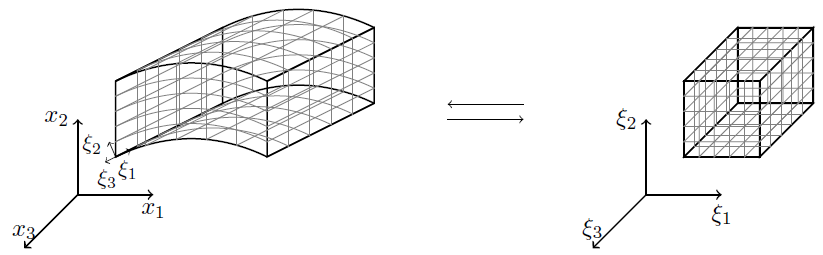
\includegraphics[height=1.8in]{coordinate_transform}
 \caption{Representation of coordinate transformation from Cartesian physical space (left) to a curvilinear orthogonal computational space (right), figure taken from \citet{munsch2015entwicklung}}
 \label{fig:3.1}
\end{figure}

The differential operators of the curvilinear coordinate domain is given by:

\begin{align}
 d\xi &= \frac{\partial{\xi}}{\partial{x}}dx+\frac{\partial{\xi}}{\partial{y}}dy+\frac{\partial{\xi}}{\partial{z}}dz\\
 d\eta &= \frac{\partial{\eta}}{\partial{x}}dx+\frac{\partial{\eta}}{\partial{y}}dy+\frac{\partial{\eta}}{\partial{z}}dz\\
 d\zeta &= \frac{\partial{\zeta}}{\partial{x}}dx+\frac{\partial{\zeta}}{\partial{y}}dy+\frac{\partial{\zeta}}{\partial{z}}dz
\end{align}

Similarly the reverse transformation from curvilinear space to the Cartesian space is denoted as follows.
\begin{align}
 x &= x\left(\xi,\eta,\zeta\right)\\
 y &= y\left(\xi,\eta,\zeta\right)\\
 z &= z\left(\xi,\eta,\zeta\right)
\end{align}

The total differential operators for reverse transformation is given by the following terms.

\begin{align}
 dx &= \frac{\partial{x}}{\partial{\xi}}d\xi+\frac{\partial{x}}{\partial{\eta}}d\eta+\frac{\partial{x}}{\partial{\zeta}}d\zeta\\
 dy &= \frac{\partial{y}}{\partial{\xi}}d\xi+\frac{\partial{y}}{\partial{\eta}}d\eta+\frac{\partial{y}}{\partial{\zeta}}d\zeta\\
 dz &= \frac{\partial{z}}{\partial{\xi}}d\xi+\frac{\partial{z}}{\partial{\eta}}d\eta+\frac{\partial{z}}{\partial{\zeta}}d\zeta
\end{align}

Both the transformations can be represented in a matrix notation as given by the following set of equations.

\begin{equation}
%\[
\begin{pmatrix}
d\xi\\
d\eta\\
d\zeta
\end{pmatrix}
=
\begin{pmatrix}
\frac{\partial{\xi}}{\partial{x}} & \frac{\partial{\xi}}{\partial{y}} & \frac{\partial{\xi}}{\partial{z}}\\
\frac{\partial{\eta}}{\partial{x}} & \frac{\partial{\eta}}{\partial{y}} & \frac{\partial{\eta}}{\partial{z}}\\
\frac{\partial{\zeta}}{\partial{x}} & \frac{\partial{\zeta}}{\partial{y}} & \frac{\partial{\zeta}}{\partial{z}}\\
\end{pmatrix}
\begin{pmatrix}
dx\\
dy\\
dz
\end{pmatrix}
%\]
\label{eqn:3.13}
\end{equation}

\begin{equation}
%\[
\begin{pmatrix}
dx\\
dy\\
dz
\end{pmatrix}
=
\begin{pmatrix}
\frac{\partial{x}}{\partial{\xi}} & \frac{\partial{x}}{\partial{\eta}} & \frac{\partial{x}}{\partial{\zeta}}\\
\frac{\partial{y}}{\partial{\xi}} & \frac{\partial{y}}{\partial{\eta}} & \frac{\partial{y}}{\partial{\zeta}}\\
\frac{\partial{z}}{\partial{\xi}} & \frac{\partial{z}}{\partial{\eta}} & \frac{\partial{z}}{\partial{\zeta}}\\
\end{pmatrix}
\begin{pmatrix}
d\xi\\
d\eta\\
d\zeta
\end{pmatrix}
%\]
\label{eqn:3.14}
\end{equation}

The matrices in the equations \ref{eqn:3.13} and \ref{eqn:3.14} are termed as transformation or \textit{Jacobian} matrices. The matrices are referenced as $a_{ij}$ and $b_{ij}$ respectively for easier notation. In general applications the computational grid is generated in the physical space. The relations in mapping to the curvilinear space as given by the set of equations \ref{eqn:3.1} are unknown and consequently the transformation matrix $a_{ij}$ as represented in the equation \ref{eqn:3.13} is also unknown. 

The transformation matrix $a_{ij}$ can be calculated from the following relationship:

\begin{equation}
\begin{pmatrix}
\frac{\partial{\xi}}{\partial{x}} & \frac{\partial{\xi}}{\partial{y}} & \frac{\partial{\xi}}{\partial{z}}\\
\frac{\partial{\eta}}{\partial{x}} & \frac{\partial{\eta}}{\partial{y}} & \frac{\partial{\eta}}{\partial{z}}\\
\frac{\partial{\zeta}}{\partial{x}} & \frac{\partial{\zeta}}{\partial{y}} & \frac{\partial{\zeta}}{\partial{z}}\\
\end{pmatrix} 
=
\begin{pmatrix}
\frac{\partial{x}}{\partial{\xi}} & \frac{\partial{x}}{\partial{\eta}} & \frac{\partial{x}}{\partial{\zeta}}\\
\frac{\partial{y}}{\partial{\xi}} & \frac{\partial{y}}{\partial{\eta}} & \frac{\partial{y}}{\partial{\zeta}}\\
\frac{\partial{z}}{\partial{\xi}} & \frac{\partial{z}}{\partial{\eta}} & \frac{\partial{z}}{\partial{\zeta}}
\end{pmatrix}^{-1}
\label{eqn:3.15}
\end{equation}
This can also be represented using referenced notation as 
\begin{equation}
\left(a_{ij}\right) = \left(b_{ij}\right)^{-1}
\label{eqn:3.16}
\end{equation}

The inverse of the transformation matrix $b_{ij}$ is calculated as represented below in the equation \ref{eqn:3.17}.
\begin{equation}
\left(a_{ij}\right) = \left(b_{ij}\right)^{-1} = \frac{adj\left(b_{ij}\right)}{\det\left(b_{ij}\right)} 
\label{eqn:3.17}
\end{equation}	
where, $adj\left(b_{ij}\right)$ is the transpose of the cofactor matrix of $\left(b_{ij}\right)$ and the determinant of the transformation matrix is the \textit{Jacobian} and is denoted by J. Thus, the inverse of the transformation matrix can be rewritten as 
\begin{equation}
\left(b_{ij}\right)^{-1} = \frac{1}{J}
\begin{pmatrix}
\beta_{11} & \beta_{12} & \beta_{13}\\
\beta_{21} & \beta_{22} & \beta_{23}\\
\beta_{31} & \beta_{32} & \beta_{33}
\end{pmatrix}
\label{eqn:3.18}
\end{equation}
where the coefficients are calculated as 
\begin{align}
\beta_{11} &= \frac{\partial{y}}{\partial{\eta}}\frac{\partial{z}}{\partial{\zeta}} - \frac{\partial{y}}{\partial{\zeta}}\frac{\partial{z}}{\partial{\eta}} = \frac{\partial{\xi}}{\partial{x}}J\\
	\beta_{12} &= \frac{\partial{x}}{\partial{\zeta}}\frac{\partial{z}}{\partial{\eta}} - \frac{\partial{x}}{\partial{\eta}}\frac{\partial{z}}{\partial{\zeta}} = \frac{\partial{\xi}}{\partial{y}}J\\
	\beta_{13} &= \frac{\partial{x}}{\partial{\eta}}\frac{\partial{y}}{\partial{\zeta}} - \frac{\partial{x}}{\partial{\zeta}}\frac{\partial{y}}{\partial{\eta}} = \frac{\partial{\xi}}{\partial{z}}J\\
	\beta_{21} &= \frac{\partial{y}}{\partial{\zeta}}\frac{\partial{z}}{\partial{\xi}} - \frac{\partial{y}}{\partial{\xi}}\frac{\partial{z}}{\partial{\zeta}} = \frac{\partial{\eta}}{\partial{x}}J\\
	\beta_{22} &= \frac{\partial{x}}{\partial{\xi}}\frac{\partial{z}}{\partial{\zeta}} - \frac{\partial{x}}{\partial{\zeta}}\frac{\partial{z}}{\partial{\xi}} = \frac{\partial{\eta}}{\partial{y}}J\\
	\beta_{23} &= \frac{\partial{x}}{\partial{\zeta}}\frac{\partial{y}}{\partial{\xi}} - \frac{\partial{x}}{\partial{\xi}}\frac{\partial{y}}{\partial{\zeta}} = \frac{\partial{\eta}}{\partial{z}}J\\
	\beta_{31} &= \frac{\partial{y}}{\partial{\xi}}\frac{\partial{z}}{\partial{\eta}} - \frac{\partial{y}}{\partial{\eta}}\frac{\partial{z}}{\partial{\xi}} = \frac{\partial{\zeta}}{\partial{x}}J\\
	\beta_{32} &= \frac{\partial{x}}{\partial{\eta}}\frac{\partial{z}}{\partial{\xi}} - \frac{\partial{x}}{\partial{\xi}}\frac{\partial{z}}{\partial{\eta}} = \frac{\partial{\zeta}}{\partial{y}}J\\
	\beta_{33} &= \frac{\partial{x}}{\partial{\eta}}\frac{\partial{y}}{\partial{\eta}} - \frac{\partial{x}}{\partial{\eta}}\frac{\partial{y}}{\partial{\xi}} = \frac{\partial{\zeta}}{\partial{z}}J
 \label{eqn:3.19}
\end{align}

The gradients of a scalar quantity along the Cartesian coordinates are transformed via the chain rule to the curvilinear coordinate system:

\begin{equation}
 \frac{\partial\phi}{\partial{x_{i}}} = \frac{\partial\phi}{\partial{\xi_j}}\frac{\partial{\xi_j}}{\partial{x_i}} = \frac{\partial\phi}{\partial{\xi_j}}\frac{\beta_{ij}}{J}
 \label{eqn:3.28}
\end{equation}

The divergence of a vector quantity $\phi_{i}$ can be calculated as follows:
\begin{equation}
\frac{\partial{\phi_i}}{\partial{x}} = \frac{\partial{\phi_{i}}}{\partial{\xi_{j}}}\frac{\beta_{ij}}{J}
\label{eqn:3.29}
\end{equation}

The Laplacian of a scalar quantity is represented in the computational space as defined below.

\begin{equation}
\frac{\partial}{\partial{x_i}}\left(\frac{\partial\phi}{\partial{x_i}}\right) = \frac{\partial}{\partial{\xi_j}}\left(\frac{\partial\phi}{\partial{\xi_k}}\frac{\beta_{ki}}{J}\frac{\beta_{ji}}{J}\right)
\label{eqn:3.30}
\end{equation}

In a Cartesian coordinate or physical space, the general transport equation for an \textit{incompressible Newtonian fluid} with a transport variable $\Phi$ is represented as,
\begin{equation}
\frac{\partial{\left(\rho\Phi\right)}}{\partial{t}}+\frac{\partial{\left({\rho}{u_i}\Phi\right)}}{\partial{x_i}} = \frac{\partial}{\partial{x_i}}\left(\Gamma_{\Phi}\frac{\partial{\Phi}}{\partial{x_i}}\right)+S_{\Phi}
\label{eqn:3.31}
\end{equation}
where the source term $S_{\Phi}$ is represented as follows.
\begin{equation}
S_{\Phi} = -\frac{\partial{p}}{\partial{x_i}}+{\rho}gi
\end{equation}

In the equation \ref{eqn:3.31}, the term $\Gamma_{\Phi}$ represents the diffusion coefficient of the transport equation. The transformed equation in curvilinear or computational space is represented based on the gradient, divergence and Laplacian as represented in the equations \ref{eqn:3.28}, \ref{eqn:3.29} and \ref{eqn:3.30} respectively. 
\begin{equation}
\frac{\partial{\left(\rho\Phi\right)}}{\partial{t}}+\frac{1}{J}\frac{\partial{\left({\rho}{U_j}{\Phi}J\right)}}{\partial{\xi_j}} = \frac{1}{J}\frac{\partial}{\partial{\xi_j}}\left(\frac{\Gamma_{\Phi}}{J}\frac{\partial{\Phi}}{\partial{\xi_k}}B_{kj}\right)+S_{\Phi}
\label{eqn3.33}
\end{equation}

The transformed source term in curvilinear coordinate system is represented as,
\begin{equation}
S_{\Phi} = -\frac{1}{J}\left(\frac{\partial{p}}{\partial{\xi_k}}\beta_{ki}\right)+{\rho}gi
\end{equation}

The velocity component $U_j=\left(U,V,W\right)$ describes the \textit{contravariant velocity} components which are based on the metric coefficients $\beta_{ij}$, the Jacobian J and the respective Cartesian velocity components. They can be evaluated as follows.
\begin{equation}
U_j = \frac{1}{J}\left(u{\beta_{j1}}+v{\beta_{j2}}+w{\beta_{j3}}\right)=\frac{1}{J}\left(u_{n}{\beta_{jn}}\right)
\end{equation}

The coefficients $B_{kj}$ are described as:
\begin{equation}
B_{kj} = \beta_{km}\beta_{jm} = \beta_{k1}\beta_{j1}+\beta_{k2}\beta_{j2}+\beta_{k3}\beta_{j3}
\label{eqn:3.36}
\end{equation}

If the grid is orthogonal in the physical space, the off-diagonal elements $\beta_{ij}$ in the transformation tensor vanishes and the general equation will be similar to the Cartesian form. The elements $b_{ij}$ can be approximated at the control volume (CV) centers using second order central difference scheme.
\begin{equation}
\left(b_{ij}\right)_P = \left(\frac{\partial x_i}{\partial \xi}\right)_P \approx \frac{x_{i,e} - x_{i,w}}{\delta \xi}
\label{eqn:3.37}
\end{equation}
The distance between the centers of the control volumes is assumed to be 1, i.e. $\delta \xi = 1$. The $j^{th}$ column elements of $b_{ij}$ for the control volume represented in figure \ref{fig:3.2} can be represented as follows:
\begin{figure}[h]
\centering
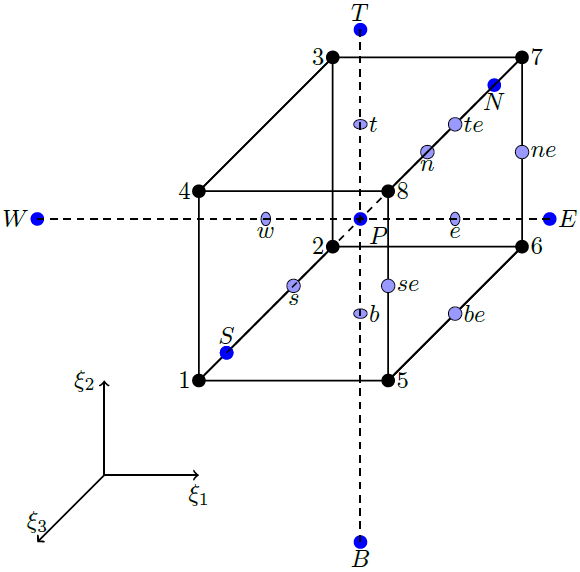
\includegraphics[height=3.5in]{cv}
\caption{Representational control volume in the computational domain, picture taken from \citet{munsch2015entwicklung}}
\label{fig:3.2}
\end{figure}

\begin{align}
	\left(b_{i1}\right)_P &= \left(\frac{\partial x_i}{\partial \xi}\right)_P \approx \frac{x_{i,5} + x_{i,6} + x_{i,7} + x_{i,8}}{4} - \frac{x_{i,1} + x_{i,2} + x_{i,3} + x_{i,4}}{4}\\
	\left(b_{i2}\right)_P &= \left(\frac{\partial x_i}{\partial \eta}\right)_P \approx \frac{x_{i,3} + x_{i,4} + x_{i,7} + x_{i,8}}{4} - \frac{x_{i,1} + x_{i,2} + x_{i,5} + x_{i,6}}{4}\\
	\left(b_{i3}\right)_P &= \left(\frac{\partial x_i}{\partial \zeta}\right)_P \approx \frac{x_{i,1} + x_{i,4} + x_{i,5} + x_{i,8}}{4} - \frac{x_{i,2} + x_{i,3} + x_{i,6} + x_{i,7}}{4}
	\label{eqn:3.40}
\end{align}

The numerical treatment of the governing equation is done by Finite volume method. The discretization of the equation is presented in the following section.

\section{Finite Volume method to solve the Navier Stokes equation}

The transformed transport equation in the conservative form is represented in the following equation. 
\begin{equation}
\int_{V_{\xi}} \frac{\partial \Phi}{\partial t}J dV_{\xi} + \int_{V_{\xi}} \frac{\partial \left(U_j \Phi\right)}{\partial \xi_j} dV_{\xi} = \int_{V_{\xi}} \frac{1}{J} \left(\Gamma_{\Phi} \frac{\partial \Phi}{\partial \xi_k} B_{kj} \right) dV_{\xi} + \int_{V_{\xi}} JS_{\Phi} dV_{\xi}
\label{eqn:3.41}
\end{equation}

The control volume $\left(CV\right)$ in the computational domain is related to a CV in physical domain as given below.
\begin{align}
dV_{\xi} &= d \xi d \eta d \zeta = 1\\
dV &= dx dy dz = J d \xi d \eta d \zeta = J
\label{eqn:3.43}
\end{align}

Applying the \textit{Gauss divergence} to the equation \ref{eqn:3.41}, the volume integral of the fluxes are transformed to the surface integral and the equation is rewritten as: 

\begin{equation}
\int_{V_{\xi}} \frac{\partial \Phi}{\partial t}J dV_{\xi} + \int_{A_{\xi}} U_j \Phi dA_{{\xi}_j} = \int_{A_{\xi}} \frac{1}{J} \left(\Gamma_{\Phi} \frac{\partial \Phi}{\partial \xi_k} B_{kj} \right) dA_{{\xi}_j} + \int_{V_{\xi}} JS_{\Phi} dV_{\xi}
\label{eqn:3.44}
\end{equation}

where, $A_{{\xi}_j}$ is the area vectors of the control volume surfaces. 

\subsection{Formulation of Arbitrary Lagrangian-Eulerian equation}
In FSI applications, the transport equation \ref{eqn:3.33} needs to be modified to account for the grid movement phenomena. The time coordinate has to be transformed in a way similar to the space transformation in the case of moving grids. The transformation of the time derivative is obtained as follows.

\begin{equation}
\left(\frac{\partial \Phi}{\partial t}\right)_{\xi} = \left(\frac{\partial \Phi}{\partial t}\right)_{x} + \frac{\partial \Phi}{\partial x_i} \left(\frac{\partial x_i}{\partial t}\right)_{\xi}
\label{eqn:3.45}
\end{equation}

where $\left(\frac{\partial x_i}{\partial t}\right)_{\xi}$ is the \textit{grid velocity} $\left(U_{i}^{g} \right)$. Substituting this back in the equation \ref{eqn:3.45},
\begin{equation}
\left(\frac{\partial \Phi}{\partial t}\right)_{\xi} = \left(\frac{\partial \Phi}{\partial t}\right)_{x} + \left(U_{i}^{g} \right) \frac{\partial \Phi}{\partial x_i}
\label{eqn:3.46} 
\end{equation}

The term $ \left(\frac{\partial \Phi}{\partial t}\right)_{x}$ can be expressed as a total derivative of variable $\Phi$ with respect to time $t$.

\begin{equation}
\left(\frac{\partial \Phi}{\partial t}\right)_{\xi} = \frac{1}{J} \frac{d\left(J \Phi\right)}{dt} + \left(U_{i}^{g} \right) \frac{\partial \Phi}{\partial x_i}
\label{eqn:3.47} 
\end{equation}

The equation \ref{eqn:3.47} is referred to as \textit{Arbitrary Lagrangian-Eulerian} (ALE) equation for moving grid. The conservative form of the ALE is obtained by \textit{Space Conservation Law} (SCL) which was proposed by \citet{demirdvzic1988space}. The principle behind this formulation ensures the rate of change of volume in the physical domain is consistent with the net volume flux due to the grid movement. The SCL formulation is as given below.

\begin{equation}
\int_{V_{\xi}} \frac{dJ}{dt}dV_{\xi}-\int_{A_{\xi}} U_{i}^{g} dA_{x_{i}} = 0
\label{eqn:3.48} 
\end{equation}

The general transport equation is rewritten substituting these formulations as given below.

\begin{equation}
\int_{V_{\xi}} \frac{d \Phi}{dt}J dV_{\xi} + \int_{A_{\xi}} \left(U_j-U_{i}^{g}\right) \Phi dA_{{\xi}_j} = \int_{A_{\xi}} \frac{1}{J} \left(\Gamma_{\Phi} \frac{\partial \Phi}{\partial \xi_k} B_{kj} \right) dA_{{\xi}_j} + \int_{V_{\xi}} JS_{\Phi} dV_{\xi}
\label{eqn:3.49} 
\end{equation}

In the above equation $U_{i}^{g}$ is the normal volume flux due to the grid movement. This is computed by the space conservation law.

\section{Discretization schemes for the terms in Navier Stokes equation}
The grid arrangement is considered to be \textit{collocated} arrangement where the variables are stored at the cell centers. Interpolation is applied, when the variable values are required at the cell faces. For any particular CV, the values from its neighboring control volumes are used to evaluate the variable values. This is represented in the equation below.

\begin{equation}
A_p \Phi_p + \sigma_{i=E,W,N,S,T,B} A_i \Phi_{i} = Q_{\xi}
\label{eqn:3.50} 
\end{equation}

where $A_p$ is the contribution of fluxes and other terms at the cell center and $A_i$ is the contribution of the corresponding neighbor nodes. The subsequent section deals with the discretization of each term in the transport equation \ref{eqn:3.49}.

\subsection{Discretization of convective fluxes}
The integration of the convective fluxes for a CV, is calculated by summing up the fluxes over all the faces $\left(f = e,w,s,n,t,b\right)$ of the CV. This is represented in the equation below.

\begin{equation}
\int_{A_{\xi}} U_j \Phi A d{A_{\xi}}_j \approx \sum_{f} \left(U_j \Phi \Delta {A_{\xi}}_j \right)_f \approx \sum_{f} F_f \Phi_f
\label{eqn:3.51}
\end{equation}

F is the convective mass flux through the CV faces. Integral values of the mass fluxes are approximated by \textit{mid-point rule} of integration. Example calculation of fluxes through the faces e,n and t boundary faces are represented below.

\begin{align}
F_e &= \left(u \beta_{11} + v \beta_{21} + w \beta_{31}\right)_e\\
F_n &= \left(u \beta_{12} + v \beta_{22} + w \beta_{32}\right)_n\\
F_t &= \left(u \beta_{13} + v \beta_{23} + w \beta_{33}\right)_t
\label{eqn:3.54}
\end{align}

In order to obtain the fluxes at the CV faces, interpolation is done. To improve the approximation of the convective fluxes, a deferred corrective approach for flux-blending, proposed by \citet{khosla1974diagonally} is implemented in the solver. The principal idea of flux-blending is to combine the advantage of higher order accurateness of Central Difference Scheme (CDS) avd the better robustness and boundedness of Upwind Discretization Scheme (UDS). The flux-blending scheme is represented as given below.

\begin{equation}
\left(\Phi_{e}\right)^{i+1} = \left(\Phi_{e}^{UDS}\right)^{i+1} + \alpha \left(\Phi_{e}^{CDS} - \Phi_{e}^{UDS} \right)^i
\label{eqn:3.55}
\end{equation}

In the above equation, $i$ is the iteration counter and $\alpha$ is the flux-blending factor. 

\subsection{Discretization of diffusive fluxes and source term}

The diffusive fluxes are generally split into \textit{orthogonal} and \textit{non-orthogonal} parts due to the grid non-orthogonality. The orthogonal part of the diffusive fluxes at the face $'e'$ and direction $\xi$ can be represented as follows.

\begin{equation}
F_{e,O}^d = \left(\Gamma_{\Phi} \frac{\partial \Phi}{\partial {\xi_i}} \frac{B_{11}}{J} \right)_e \approx \left(\frac{\partial \Phi}{J} \right)_e \left(\Phi_E - \Phi_P \right) \left(\beta_{11} \beta_{11} + \beta_{21} \beta_{21}+ \beta_{31} \beta_{31} \right)_e
\label{eqn:3.56}
\end{equation}

The orthogonal part of the diffusive fluxes can be computed similarly in the other directions. The non-orthogonal part of the diffusive fluxes are treated explicitly, so that the size of the coefficient matrix can be restricted. The non-orthogonal part of the diffusive fluxes at face $'e'$ can be computed as shown below.

\begin{align}
 F_{e,NO}^d = \frac{1}{J} \left(\Gamma_{\Phi} B_{12} \frac{\partial \Phi}{\partial {\eta}} + \Gamma_{\Phi} B_{13} \frac{\partial \Phi}{\partial {\zeta}} \right)_e\\
 \left(\frac{\partial \Phi}{\partial {\eta}} \right)_e \approx \Phi_{ne} - \Phi_{se}\\
 \left(\frac{\partial \Phi}{\partial {\zeta}} \right)_e \approx \Phi_{te} - \Phi_{be}
\label{eqn:3.59}
\end{align}

The unknown fluxes at the CV corner points are interpolated by a weighted linear interpolation technique. The approximation of the source term is carried out by mid-point rule of integration as follows:

\begin{equation}
\int_{V_{\xi}} J S_{\Phi} dV_{\xi} \approx \left(S_{\Phi} J \right)_P
\label{eqn:3.60}
\end{equation}

\subsection{Time discretization scheme}
The FASTEST-3D solver has various time discretization schemes such as \textit{Implicit Euler scheme, Crank-Nicholson method (implicit in nature), and 3 steps and 5 steps explicit Runge-Kutta methods}. For the current study, 3-step second order accurate Runge-Kutta method has been used. Low storage variants of the Runge-Kutta method proposed by \citet{williamson1980low} has been implemented in the solver. The explicit time marching scheme for momentum equation discretization is represented in the following set of equations. 

\begin{align}
u_i^1 & = u_i^n + \alpha_1 \frac{\Delta t}{\rho V} R\left(u_i^n\right) ; \alpha_1 = \frac{1}{3}\\
u_i^2 & = u_i^n + \alpha_2 \frac{\Delta t}{\rho V} R\left(u_i^1\right) ; \alpha_2 = \frac{1}{2}\\
u_i^3 & = u_i^n + \alpha_3 \frac{\Delta t}{\rho V} R\left(u_i^2\right) ; \alpha_3 = 1\\
u_i^{\star} &= u_i^3
\label{eqn:3.64}
\end{align}

The cell volume is initially assumed to be constant, and $R(\Phi)$ is defined as: 

\begin{equation}
\frac{d}{dt} \int_{{V}_{\xi}} \Phi J d_{{V}_{\xi}} = R\left(\Phi\right)
\label{eqn:3.65}
\end{equation}

The velocity $u^{\star}$ obtained from the equation \ref{eqn:3.64} does not satisfy the \textit{mass conservation} and is a prediction $u^{n+1}$ for the next time step. The equation is modified for moving grids and is represented by the following set of equations.

\begin{align}
u_i^1 & = \left(u_i^n V^n + \alpha_1 \frac{\Delta t}{\rho} R\left(u_i^n \right) \right) \frac{1}{V^n + \alpha_1 \left(V^{\left(n+1\right)} - V^n \right)}\\
u_i^2 & = \left(u_i^n V^n + \alpha_2 \frac{\Delta t}{\rho} R\left(u_i^1 \right) \right)\frac{1}{V^n + \alpha_2 \left(V^{\left(n+1\right)} - V^n \right)}\\
u_i^3 & = \left(u_i^n V^n + \alpha_3 \frac{\Delta t}{\rho} R\left(u_i^2 \right) \right)\frac{1}{V^n + \alpha_3 \left(V^{\left(n+1\right)} - V^n \right)}\\
u_i^{\star} &= u_i^3
\label{eqn:3.69}
\end{align}

where, $V^n$ and $V^{\left(n+1\right)}$ are the volume at time step $n$ and $n+1$ respectively. The co-efficient $\alpha_k$ is approximated according to the equation:

\begin{equation}
\alpha_k = \frac{1}{N-(k+1)}; k=1,2,3,\ldots,N
\label{eqn:3.70}
\end{equation}

\subsection{Discretization of Space Conservation Law}
The fluxes due to the grid movement is satisfied by the SCL as described in \ref{eqn:3.47}. The SCL must be satisfied in order to overcome the problem of \textit{artificial mass source} in the discretized equation. The discretization of the SCL for first and second order time integration schemes are represented below.

\begin{equation}
\sum_f \left(U_i^g \Delta A_{\xi_j} \right)_f = \frac{\Delta V^{\left(n+1\right)}- \Delta V^n}{\Delta t}
\label{eqn:3.71}
\end{equation}

The second order time integration scheme is represented as:
\begin{equation}
\sum_f \left(U_i^g \Delta A_{\xi_j} \right)_f = \frac{3 \Delta V^{\left(n+1\right)}- 4 \Delta V^n + \Delta V^{\left(n-1\right)}}{2 \Delta t}
\label{eqn:3.72}
\end{equation}

\begin{figure}[h]
\centering
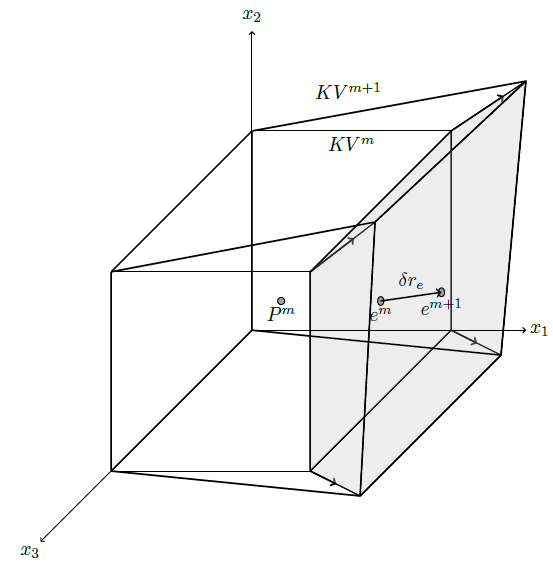
\includegraphics[height=3.2in]{swept_volume}
\caption{Representation of change in control volume due to the grid movement}
\label{fig:3.3}
\end{figure}

Figure \ref{fig:3.3} represents an arbitrary control volume and a change in volume due to the grid movement. The fluxes due to the movement of the east face can be calculated as :

\begin{equation}
\left(U_i^g \Delta A_{\xi_j} \right)_e \approx \Phi_e \frac{3\left(\partial V\right)_e^{n+1}-\left(\partial V \right)_e^{n}}{2 \Delta t}
\end{equation}

\subsection{Mass conservation (Pressure-Velocity coupling)}

As explained previously, the velocity obtained by the 3 step Runge-Kutta method does not satisfy the mass conservation as the velocity is not divergence free. To alleviate this concern, the Pressure-Velocity coupling scheme is implemented. In the current solver a predictor corrector approach as proposed by \citet{munsch2015entwicklung} has been implemented. This approach is explained below.
\begin{itemize}
\item Prediction step: The provisional velocity field $u_i^{\star}$ is determined by the 3 step Runge-Kutta discretization method.
\item Pressure Poission equation: A pressure correction term $\acute{p} = p^{n+1} - p^{\star}$ is computed and in-turn the magnitude of velocity correction $\acute{u_i}$ is computed.
\item Correction step: The pressure and velocity obtained in the previous step is used to correct the respective values. The obtained velocity is now divergence free and satisfies mass conservation.
\end{itemize}

\subsubsection{Pressure Poisson equation}
The semi discretized momentum equation based on the approximate velocity quantity $u_i^{\star}$ and the velocity prediction for next time step $u_i^{n+1}$ in Cartesian system is represented as follows:

\begin{align}
\rho \frac{u_i^{\star} - u_i^n}{\Delta t} &= - \left[ \frac{\partial \left(\rho u_i u_j \right)}{\partial x_j} \right]^n + \left[ \frac{\partial}{\partial x_j} \left(\Gamma \frac{\partial u_i}{\partial x_j} \right) \right]^n - \left[\frac{\partial p}{\partial x_j} \right]^{\star}\\
\rho \frac{u_i^{n+1} - u_i^n}{\Delta t} &= - \left[ \frac{\partial \left(\rho u_i u_j \right)}{\partial x_j} \right]^n + \left[ \frac{\partial}{\partial x_j} \left(\Gamma \frac{\partial u_i}{\partial x_j} \right) \right]^n - \left[\frac{\partial p}{\partial x_j} \right]^{n+1}
\label{eqn:3.74}
\end{align}

The difference between the equations mentioned above yields,

\begin{equation}
u_i^{n+1} - u_i^{\star} = - \frac{\Delta t}{\rho} \left[ \frac{\partial p^{n+1}}{\partial x_j} - \frac{\partial p^{\star}}{\partial x_j} \right]
\label{eqn:3.75}
\end{equation}

divergence of the equation \ref{eqn:3.75} is taken, which approximates to:

\begin{equation}
\frac{\partial u_i^{\star}}{\partial x_i} = \frac{\Delta t}{\rho} \frac{\partial}{\partial x_i} \left[ \frac{\partial p^{n+1}}{\partial x_j} - \frac{\partial p^{\star}}{\partial x_j} \right]
\label{eqn:3.76}
\end{equation}

The above equation can be simplified using the relation $\acute{p} = p^{n+1} - p^{\star}$,

\begin{equation}
\frac{\partial u_i^{\star}}{\partial x_i} = \frac{\Delta t}{\rho} \frac{\partial}{\partial x_i} \left[ \frac{\partial \acute{p}}{\partial x_i} \right]
\label{eqn:3.77}
\end{equation}

The Poisson equation \ref{eqn:3.77} is represented in computational domain as given below.

\begin{equation}
\left[ \frac{\partial}{\partial {\xi_j}} \left(J U_j^{\star} \right) \right] = \frac{\Delta t}{\rho} \frac{\partial}{\partial {x_j}} \left[ \frac{\partial \acute{p}}{\partial {\xi_j}} \frac{1}{J} \beta_{ki} \beta_{ji} \right] 
\label{eqn:3.78}
\end{equation}

In FASTEST-3D solver, \textit{Strongly Implicit Procedure (SIP solver)} is implemented to solve the Poisson equation. SIP is an incomplete lower-upper decomposition method (ILU) which is specially designed for algebraic equations that are discretizations of partial differential equations and does not apply to generic system of equations. Detailed explanation of implementation can be found in \citet{munsch2015entwicklung}. 

\section{Discretization of the structural governing equation}

The time integration of the structure governing equation is done by \textit{generalized-$\alpha$} method which was proposed by \citet{chung1993time}. The matrix equation for the linear structural equation of linear structural dynamics is given by the following equation.

\begin{equation}
M\ddot{d} + C\dot{d} + Kd = F
\label{eqn:3.79}
\end{equation}

In the equation \ref{eqn:3.79}, $M$, $C$, and $K$ represents the mass, damping co-efficient and stiffness matrices respectively. $F$ represents the vector of forces acting on the structure. $d$ is the vector of unknown displacements, $\dot{d} = v$ the velocity and $\ddot{d} = a$ the acceleration of the structure. This is an initial-value problem for finding the displacement $d = d(t)$ with the initial values:

\begin{align}
d(0) &= d_0\\
\dot{d}_0 &= v_0
\label{eqn:3.81}
\end{align}

The generalized-$\alpha$ method can be represented as:
\begin{align}
d_{n+1} &= d_n + \partial t v_n + \delta t^{2} \left(\left( \frac{1}{2} - \beta \right) a_n + \beta a_{n+1} \right)\\
v_{n+1} &= v_n + \delta t \left(\left( 1 - \gamma \right) a_n + \gamma a_{n+1} \right)\\
M_{a_{n+1,\alpha_m}} + C {v_{n+1,\alpha_f}} + K {d_{n+1,\alpha_f}} &= F \left( t_{n+1,\alpha_f} \right)
\label{eqn:3.84}
\end{align}

where $a_0 = M^{-1} \left(F(0) - Cv_0 - Kd \right)$. 

\begin{align}
d_{{n+1},\alpha_f} &= \left(1-{\alpha_f}\right)d_{n+1} + \alpha_f d_n\\
v_{{n+1},\alpha_f} &= \left(1-{\alpha_f}\right)v_{n+1} + \alpha_f v_n\\
a_{{n+1},\alpha_m} &= \left(1-{\alpha_m}\right)a_{n+1} + \alpha_m a_n\\
t_{{n+1},\alpha_f} &= \left(1-{\alpha_f}\right)t_{n+1} + \alpha_f t_n
\label{eqn:3.88}
\end{align}

In the above set of equations \ref{eqn:3.88}, $\alpha_m, \alpha_f, \gamma, and, \beta$ are real valued approximations that define the time integration scheme. The generalized-$\alpha$ method is second order accurate and is unconditionally stable if the following condition is satisfied.

\begin{align}
\alpha &= \frac{1}{2} + \alpha_m - \alpha_f\\
\alpha_m &\leq \alpha_f \leq \frac{1}{2}\\
\beta &= \frac{1}{4} \left(1 - \alpha_m + \alpha_f \right)^2
\label{eqn:3.91}
\end{align} 

To have a control over the high-frequency dissipation, $\alpha_m$ and $\alpha_f$ are normalized by the spectral radius of the amplification matrix $\rho_{\infty}$.

\begin{align}
\alpha_m &= \frac{2 - {\rho_{\infty}}}{1 + {\rho_{\infty}}}\\
\alpha_f &= \frac{1}{1 + {\rho_{\infty}}}
\label{eqn:3.93}
\end{align}

The spectral radius $\rho_\infty$ is bounded by the following condition.

\begin{equation}
\frac{1}{3} \leq \lVert{\frac{-1 -3 \rho_{\infty}}{3+ \rho_{\infty}}}\rVert \leq 1; \forall \lVert{\rho_{\infty}}\rVert \leq 1
\label{eqn:3.94}
\end{equation}